\section{测量细节与附表}
\label{sec:measurement-details}
本批实验统一使用 TVM \texttt{0.26.dev90}、CUDA 12.6 与 \texttt{sm\_86} 目标，平台为 RTX 3050 Ti Laptop GPU（4 GiB）。搜索 seed 固定为 20261011，每臂 32 submitted、批大小 4、种群 32、探索比例 0.1；MatMul128 分别设置 1 与 4 代 GA，其余为 1 代。代价模型为 XGBoost、warmup 0；D 的入围比例 \texttt{verify\_ratio}=0.25。每个候选在计时前通过独立缓冲的数值检查（与 NumPy FP64 参考比对，rtol=atol=$2\times10^{-4}$）；完整调优时间从 Tune 开始到返回，含 search、builder、runner 与 callback，准备时间单列。

15 次运行、480 次提交均获得有限且数值正确的测量。Windows 上完成测量后的进程退出异常通过 worker 规避处理，未宣称根因修复。表~\ref{tab:single-primary} 报告生成/Verify 与时间，表~\ref{tab:single-ga} 报告 GA 密度下的评分开销，表~\ref{tab:single-targets} 报告全部目标阈值；图~\ref{fig:single-retiming} 给出原 top-1 独立重测的完整分布。

% Auto-generated from audited summary.json; do not edit numeric cells.
% Source SHA256: 32b22c8a529af34f8b22a9bfd7397a15e93341e689830e89ff46a5cdcd1cc663
% Regenerate with experiments/export_single_seed_paper_tables.py.
\begin{table*}[tb]
\centering
\caption{同预算主结果：预先固定一个搜索 seed（20261011），每臂 32 submitted，均得到 32 次有限且正确的测量。B=baseline，C=CS+H，D=CS+H+粗筛。观测最优来自调优数据库；重测固定原 top-1，每臂 30 个技术重复的中位数，不回填调优曲线，也不增加独立搜索 seed。}
\label{tab:single-primary}
\fontsize{9}{11}\selectfont
\setlength{\tabcolsep}{4pt}
\begin{tabular}{llrrrrrr}
\toprule
算子 / GA & 臂 & 生成 & \shortstack{Verify\\失败} & \shortstack{Search\\(s)} & \shortstack{Tune\\(s)} & \shortstack{观测最优\\($\mu$s)} & \shortstack{原 top-1 重测\\中位数 ($\mu$s)} \\
\midrule
MatMul128 / 1 & B & 2018 & 1531 & 105.154 & 790.161 & 34.0845 & 31.7013 \\
 & C & 773 & 231 & 145.273 & 778.711 & 33.6107 & 31.8705 \\
 & D & 732 & 210 & 127.051 & 773.069 & 33.5186 & 34.0597 \\
\midrule
MatMul128 / 4 & B & 3068 & 1952 & 133.155 & 765.013 & 33.0918 & 37.5262 \\
 & C & 1474 & 224 & 140.818 & 817.116 & 35.2377 & 36.1484 \\
 & D & 1535 & 274 & 143.172 & 811.631 & 33.4867 & 35.1035 \\
\midrule
MatMul256 / 1 & B & 2453 & 1966 & 136.738 & 802.983 & 32.8173 & 31.4930 \\
 & C & 1040 & 516 & 172.585 & 867.306 & 50.0943 & 44.1429 \\
 & D & 966 & 451 & 140.925 & 783.873 & 33.8304 & 34.4057 \\
\midrule
Conv / 1 & B & 1958 & 1467 & 119.082 & 794.351 & 34.3407 & 37.7946 \\
 & C & 758 & 199 & 118.814 & 809.308 & 33.7829 & 37.6410 \\
 & D & 757 & 208 & 134.831 & 834.919 & 34.9225 & 37.6904 \\
\midrule
Reduction / 1 & B & 373 & 0 & 1.353 & 665.286 & 35.7334 & 35.9612 \\
 & C & 344 & 0 & 1.376 & 665.380 & 37.2612 & 36.8367 \\
 & D & 359 & 0 & 0.816 & 628.305 & 33.5466 & 32.4199 \\
\bottomrule
\end{tabular}
\end{table*}

% Auto-generated from audited summary.json; do not edit numeric cells.
% Source SHA256: 32b22c8a529af34f8b22a9bfd7397a15e93341e689830e89ff46a5cdcd1cc663
% Regenerate with experiments/export_single_seed_paper_tables.py.
\begin{table*}[tb]
\centering
\caption{MatMul128 的 GA 密度与评分开销：同一搜索 seed，每臂 32 submitted。预测节省与 Tune 减少均比较 C（CS+H）到 D（CS+H+粗筛）；粗筛自身评分和 XGBoost 预测已嵌套于 Search，不能重复加入总 Tune。}
\label{tab:single-ga}
\small
\setlength{\tabcolsep}{4pt}
\begin{tabular}{rrrrrrr}
\toprule
GA & \shortstack{XGB 输入\\C$\to$D} & \shortstack{C 预测\\(s)} & \shortstack{D 预测\\(s)} & \shortstack{预测节省\\(s)} & \shortstack{D 粗筛评分\\(s)} & \shortstack{Tune 减少\\(\%)} \\
\midrule
1 & $512\to64$ & 2.560564 & 0.333087 & 2.227477 & 0.079086 & 0.72 \\
4 & $1280\to64$ & 6.427177 & 0.330386 & 6.096791 & 0.223606 & 0.67 \\
\bottomrule
\end{tabular}
\end{table*}

% Auto-generated from audited summary.json; do not edit numeric cells.
% Source SHA256: 32b22c8a529af34f8b22a9bfd7397a15e93341e689830e89ff46a5cdcd1cc663
% Regenerate with experiments/export_single_seed_paper_tables.py.
\begin{table*}[tb]
\centering
\caption{全部目标阈值的达标提交数 / 完整 Tune 秒数：一个搜索 seed，每臂 32 submitted。NR(截止秒数) 表示预算耗尽仍未达标。MatMul128 的 40/50\,$\mu$s 为预定目标；扩展算子的三档目标为各自 baseline 调优终点的 1/1.01/1.05 倍，属于回顾性描述。整批 callback 完成后才判定达标，不插值，准备时间单列；目标依据调优观测，独立原赢家重测不回填本表。}
\label{tab:single-targets}
\small
\setlength{\tabcolsep}{4pt}
\begin{tabular}{lrrrr}
\toprule
算子 / GA & \shortstack{目标\\($\mu$s)} & \shortstack{B\\提交 / Tune (s)} & \shortstack{C\\提交 / Tune (s)} & \shortstack{D\\提交 / Tune (s)} \\
\midrule
MatMul128 / 1 & 40.0000 & 4 / 128.634 & 4 / 118.522 & 4 / 120.822 \\
 & 50.0000 & 4 / 128.634 & 4 / 118.522 & 4 / 120.822 \\
\midrule
MatMul128 / 4 & 40.0000 & 4 / 113.543 & 24 / 628.530 & 4 / 121.206 \\
 & 50.0000 & 4 / 113.543 & 4 / 126.508 & 4 / 121.206 \\
\midrule
MatMul256 / 1 & 32.8173 & 32 / 802.979 & NR(867.306) & NR(783.873) \\
 & 33.1455 & 28 / 702.860 & NR(867.306) & NR(783.873) \\
 & 34.4582 & 12 / 312.693 & NR(867.306) & 4 / 124.729 \\
\midrule
Conv / 1 & 34.3407 & 4 / 127.076 & 4 / 126.255 & NR(834.919) \\
 & 34.6841 & 4 / 127.076 & 4 / 126.255 & NR(834.919) \\
 & 36.0577 & 4 / 127.076 & 4 / 126.255 & 20 / 554.838 \\
\midrule
Reduction / 1 & 35.7334 & 16 / 338.406 & NR(665.380) & 32 / 628.301 \\
 & 36.0907 & 16 / 338.406 & NR(665.380) & 32 / 628.301 \\
 & 37.5201 & 12 / 263.545 & 4 / 102.552 & 4 / 96.277 \\
\bottomrule
\end{tabular}
\end{table*}


\begin{figure*}[tb]
\centering
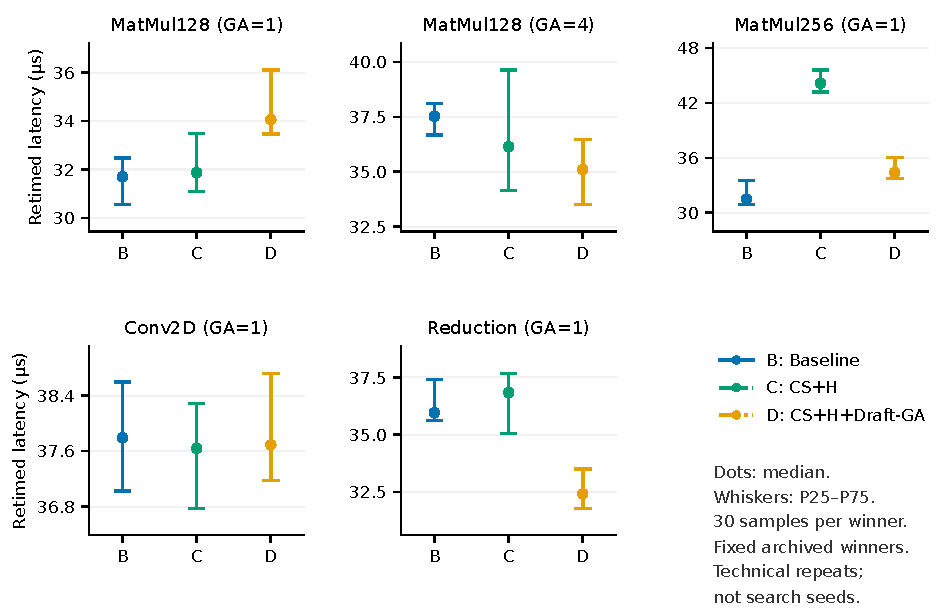
\includegraphics[width=\linewidth]{figures/single_seed_paper_20261010/f5_independent_top1.pdf}
\caption{原 top-1 候选的独立重测延迟分布。每臂 30 个技术重复，中位数用于主文比较；技术重复不增加独立搜索 seed。}
\label{fig:single-retiming}
\end{figure*}
